\documentclass[utf8]{gradu3}

\usepackage{graphicx}

%\usepackage{amsmath} % hyödyllinen jos tekstisi sisältää matikkaa,
%                     % ei pakollinen

\usepackage{biblatex}

% HUOM! Tämän tulee olla viimeinen \usepackage koko dokumentissa!
\usepackage[bookmarksopen,bookmarksnumbered,linktocpage]{hyperref}

\addbibresource{diary-4.bib}

\begin{document}

\title{ITKY4000-kurssin viimeiset hetket}
\translatedtitle{The Final Moments of ITKY4000}

\author{Mikael Myyrä}
\contactinformation{\texttt{mikael.b.myyra@jyu.fi}}
\studyline{Ohjelmisto- ja tietoliikennetekniikka}

\tiivistelma{Tämä on oppimispäiväkirjani kurssilla ITKY4000. Tässä
  kokoan yhteen, jalostan ja laajennan kolmen aiemman
  oppimispäiväkirjan sisältöjä. Pohdin tässä taustojani ja
  tavoitteitani omassa elämässäni sekä erityisesti sitä, miten
  suunnittelen yhdistäväni siihen juuri alkaneet maisteriopintoni.
}

\abstract{English abstract is not relevant for the ITKY4000 course.
  (In a thesis, it is usually an exact translation of the
  Finnish ``tiivistelmä''.)
}

\avainsanat{orientaatiokurssi, %
  HOPS, %
  omakohtainen reflektio %
}

\keywords{orientation course, %
  personal study plan, %
  self-directed reflection %
}

\supervisor{Itseohjautuva omakohtainen pohdinta}
\type{ITKY4000 -kurssin oppimispäiväkirja}
\subject{IT-opiskelijoiden}

\maketitle

\mainmatter

\sloppypar

\chapter{Johdanto}

Tämä teksti kokoaa yhteen kurssin ``ITKY4000 Yliopisto-opinnot ja
niiden suunnittelu maisterikoulutettaville'' oppimispäiväkirjan
osat. Kuvailen tässä tehtävänannon mukaisesti omia ajatuksiani
juuri aloittamieni maisteriopintojen alkuvaiheeseen liittyen.

Luvussa \ref{taustatJaTavoitteet} kuvailen lyhyesti opintohistoriani:
mistä tulen ja mihin pyrin nyt alkavien maisteriopintojen kautta.

Luvussa \ref{tapahtumaraportit} kerron, mitä ajatuksia minussa
heräsi parista lukukauden alkuviikkoina pidetystä tapahtumasta.

Luvussa \ref{kuvanPohdintaa} selitän yksityiskohtaisesti auki
oppimispäiväkirjan toisena osuutena tuottamani infografiikan.

Luku \ref{hopsJaGradu} sisältää oppimispäiväkirjan 3. osassa tekemäni
pohdinnan oman HOPSini sisällöstä sekä lukemastani pro gradu
-tutkielmasta.

Luvussa \ref{muitaAsioita} käyn omalta kohdaltani läpi vielä
oppimispäiväkirjan tehtävänannossa luetellut erityiset osa-alueet
maisteriopintoihini liittyen.

Luvussa \ref{yhteenveto} teen yhteenvedon ajatuksistani
ITKY4000-orientaatiokurssista ja maisteriopintojeni ensimmäisestä
lukukaudesta.

\chapter{Mistä tulen - mihin haluan?}
\label{taustatJaTavoitteet}

Kuten moni tietotekniikkaharrastaja, kiinnostuin aiheesta alunperin pelien
kautta. Pelien pelaamisen aloitin jo ennen kouluikää, mutta vasta
13-vuotiaana aloin ihmetellä, miten niitä oikein tehdään. Suosikkipelini oli
fysiikka\-pohjainen tasohyppely nimeltään **N**, joka on tehty
Flash-alustalle, ja sen innoittamana opettelin ohjelmoimaan ActionScript
kolmosella. Tein erittäin yksinkertaisia ja rumia pelejä, kuten
aloittelijalta voi odottaakin, mutta se oli mahdottoman hauskaa ja heti kun
tajusin, että ohjelmoija on ammatti, urasuunnitelmani oli lukkoon lyöty.

Lukion ensimmäisellä luokalla matematiikan opettajani tiesi
ohjelmointiharrastuksestani ja lähetti minut Jyväskylän yliopiston
kilpailuun, jossa palkintona oli opiskelupaikkoja. Tämähän oli kovin kätevää,
koska sinne olin päättänyt hakevani joka tapauksessa. Sain kilpailusta täydet
pisteet, miinus puolikas bonustehtävästä, jossa en tunnistanut Python-kieltä,
ja tulin ensimmäiselle sijalle. Sain opiskelupaikan ja digikameran. Pari
vuotta lukiota ja vuosi asepalvelusta myöhemmin astelin intoa puhkuen
yliopistolle. Se into on sittemmin vain kasvanut.

Eräs oleellinen muutos minäkuvassani tapahtui opintojen alkupuolella, kun
ymmärsin, miten luovaa toimintaa ohjelmointi on ja miten paljon mielihyvää
saan esteettisesti kauniista ratkaisuista. Lapsena ajattelin olevani "kylmän
analyyttinen" matemaatikkotyyppi, mutta nyt ymmärsin motivoituvani oikeastaan
enemmän luovuudesta ja kauneudesta kuin pelkästä ongelmanratkaisusta. Tämä
inspiroi kuvataide- ja musiikkiharrastuksiani ja auttoi ymmärtämään
suhdettani niin peleihin kuin myös matematiikkaan, jossa minua viehättää
ennen kaikkea sen abstrakti puhtaus yhdistettynä valtavaan ilmaisuvoimaan
käytännön todellisuudessa.

Ehdin jo kandidaatin tutkinnon loppupuolella työllistyä alalle, mutta minulle
jäi vielä niin paljon tyydyttämätöntä uteliaisuutta, että en malta jättää
käyttämättä tilaisuutta opiskella lisää. Sillä ajatuksella olen nyt
teknis-matemaattisen mallintamisen puolella — tämä on ollut minulle
harrastuneisuuden kohde jo pitkään, ja kun annetaan mahdollisuus käyttää
aiheeseen paljon aikaa ja saada vielä laadukasta opetustakin, niin onhan
sii\-hen tartuttava. Nykyiseen työhöni nähden olen täällä täysin itsekkäistä
syistä; ei tästä matematiikasta ole peruskoodaamisessa juurikaan iloa, mutta
se on hirveän hauskaa ja vieläpä hyvä tekosyy muuttaa työtä osa-aikaiseksi.
Ei ehkä pomo suostuisi, jos sanoisin vaan, että haluan tehdä harrastusjuttuja
kolmasosan työajasta. Palkka kärsii mutta pysyy riittävänä, ja onnellisuus
ottaa ison loikan.

Jossain vaiheessa kiinnostaa kyllä viedä näitä taitoja työelämäänkin esim.
pelimoottori/työkalukehityksessä tai tech-artistin hommissa pelialalla, tai
vaikka jossain tieteellisen laskennan duunissa. Jatko-opiskeluakin olen
poh\-tinut, mutta kaikkea tätä voi miettiä kunnolla sitten valmistumisen
lähestyessä. Toistaiseksi nautin hetkestä ja rahoitan opiskeluni helpolla ja
turvallisella web-kehityksellä.

\section{Kysymyksiä, joihin toivoin vastauksia} Lähinnä tässä vaiheessa
mietitytti se, miten saan opiskeluni mitoitettua sopivasti töiden ohelle.
Tiesin, miten paljon töiden päälle jää aikaa, mutta se oli toistaiseksi
tuntematon muuttuja, miten paljon siihen riittää jaksamista. Luotin kuitenkin
siihen, että parin periodin tunnustelulla tämän oppii.

Nyt kahden periodin kokemuksella voin todeta, että sain tasapainon aika hyvin
kohdalleen heti alusta lähtien. Jatkossa voin mitoittaa työmäärän
suunnitelmissani verraten tähän syksyyn.

Pieni turhautumisen aihe on, että maisteritutkinnon 120 opintopisteeseen ei
millään mahdu kaikkea mitä kiinnostaisi opiskella. Sille ei kuitenkaan tällä
kurssilla voi mitään; pitänee lähteä jatko-opiskelemaan, jos sama fiilis on
vielä tutkinnon lopulla. Oikeastaan mitään sellaista minulla ei ole mielessä,
mikä olisi ITKY4000:n puitteissa ratkaistavissa.

\chapter{Raportit lukuvuoden alkuviikkojen tapahtumista}
\label{tapahtumaraportit}

\section{Tietotekniikan ryhmätapaaminen 02.09.}

Zoomissa harjoiteltiin etätekniikan käyttöä ja tehtiin kevyitä
keskusteluharjoitteita. Juttelun aiheet liittyivät lähinnä fiiliksiin ja
odotuksiin lukukauden alussa, ja tavoite kuulosti olevan opiskelutovereihin
tutustuminen.

Itse tulin tapaamiseen varsin hämärin odotuksin; en osannut etukäteen yhtään
ajatella, minkälaista tekemistä maisteritason orientaatiokurssilla olisi, kun
oletettavasti kaikilla on korkeakouluopiskelu jo jokseenkin hanskassa. Siinä
mielessä tuntui ihan järkevältä, että tavoitteena oli juuri tutustumista ja
aktiviteettina fiiliksien jakoa.

Kuten myös tilaisuudessa mainitsin, niin aika paljon aikaa kului tekniikkaan
totutteluun ja siitä seuraavaan sähläämiseen, ja tuntui, ettei oikein mitään
substantiivista ehtinyt tapahtua. Tämä toimi kuitenkin hyvänä ensimaisteluna
Zoomin käyttöön, koska en ollut siihen juuri aiemmin koskenut. Alkukankeus
saatiin pois alta.

Olen kovin erakkoluonteinen ihminen ja toisten kanssa kasvokkain (tai
kuvakkain? kamerakkain?) keskustelu on aina vähän mukavuusalueeni
ulkopuolella, mutta oikeastaan osittain juuri siitä syystä tämä oli minulle
positiivinen kokemus. Voisin täysin tyytyväisenä pysytellä itsekseni kotona
kuukausikaupalla, ja ilman ulkopuolelta tulevia "pakotteita" (eihän tämä
varsinaisesti pakollista ole, mutta siitä saa oppimispäiväkirjaan pätkän)
varmasti tekisinkin niin, mutta vuorovaikutustaitojen ja itseluottamuksen
kannalta on hyvä välillä jutella tuntemattomienkin ihmisten kanssa.

\section{Tietotekniikan ryhmätapaaminen 16.09.}

Samaan malliin jatkettiin kuin viimeksi, mutta vähemmällä
tekniikkasählingillä. Tällä kertaa ryhmäkeskusteluissa puheenaiheina olivat
opiskeluun liittyvät riskit ja huolenaiheet sekä niiden hallintamenetelmät.
Paljon puhuttiin aikataulutuksesta ja erilaisista työkaluista ja menetelmistä
sen hallintaan. Toinen puhuttava aihe oli etätyö ja sen vaikutukset
edelliseen.

Niin aikataulutus kuin kotona työskentelykin on ollut minulla jo pitkään
hyvin hallussa, joten en varsinaisesti oppinut mitään uutta, mutta aihe on
kaikkia koskettava ja siitä oli helppo saada aikaan keskustelua. Yleisesti
ottaen tästä jäi samanlainen fiilis kuin edellisestäkin tapaamisesta; ei
mitään suuria oivalluksia, mutta hyvää vuorovaikutustreeniä. Vähän
turhauttaa, että Zoomin breakout-room-ominaisuus katkoo minulta yhteyksiä,
mutta sille ei voi kukaan mitään. Käytän melko harvinaista Linux-distroa,
jolla pitää vaan selvittää tällaiset itse tai odottaa, että joku muu tekee
sen ja julkaisee uuden paketin.


\chapter{Taitojeni verkko} \label{kuvanPohdintaa}

Kuvio \ref{verkko} esittää minulle tärkeitä taitoja ja pätevyyttäni niissä.
Jokainen sektori kuvassa on yksi taito, ja sektorin ylittävien seittirihmojen
lukumäärä kuvastaa taidon vahvuutta. Vahvimmat taitoni ovat ohjelmointi ja
opiskelu.

Metaforana tämän kuvan taustalla on turhautumiseni siitä, että kaikkien
taitojen kehittämiseen ei riitä aikaa ja energiaa. Kun keskittyy
rakentelemaan yhtä tai kahta seitin sektoria, muut pysyvät koskematta ja
rapistuvatkin vähitellen, mutta jos yrittää yltää kaikkiin, niin yhdenkään
rakentaminen ei etene nopeasti, eikä ihan kaikkia ole edes mahdollista
työstää samanaikaisesti.

Ratkaisu tähän ongelmaan on toki olemassa — tekemällä kärsivällisesti kaikkea
sopivassa suhteessa on pitkällä aikavälillä mahdollista rakentaa kaikkia
taitoja ihmisiän puitteissa kohtuullisen pitkälle. Tiedostan ja hallitsen
tämän, mutta silti se turhauttaa usein.

\begin{figure}[tp]
  \centering
  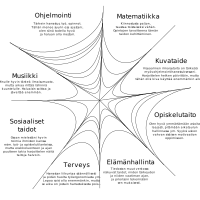
\includegraphics[width=\textwidth]{meitsi}
  \caption{\label{verkko}Taitojani kuvastava hämähäkinverkko}
\end{figure}

\chapter{Pienin askelin kohti uusien taitojen oppimista}
\label{hopsJaGradu}

\section{HOPSistani}

Tavoitteeni maisteriopinnoissa on yksinkertaisesti käyttää mahdollisimman paljon
aikaa niiden asioiden opiskeluun, jotka minua oikeasti kiinnostavat. Näitä
asioita ovat erityisesti fysiikkasimulaatiot ja tietokonegrafiikka sekä niiden
taustalla toimiva matematiikka. Yliopistossa haluan keskittyä sellaisiin
asioihin, joita en vielä osaa kovin hyvin ja joissa henkilökohtaisesta
opetuksesta on hyötyä, ja hallitsen jo ohjelmoinnin erittäin hyvin, joten
painotan HOPSissani puhdasta matematiikkaa.

Alkuun tarvitsen hieman täydennystä matematiikan aineopinnoista, että ymmärrän
fysiikan osittaisdifferentiaaliyhtälöitä ja grafiikan lineaarialgebraa. Tätä
varten olen valikoinut mukaan vektoricalculusta ja matriisilaskentaa. Sitten
alkaa pääaineen puolelta teknis-matemaattisen mallintamisen opintosuunta, jonka
sisältö on pitkälti suoraan juuri sitä, mitä haluankin opiskella.

Valinnaisissa syventävissä opinnoissa minulla on lähinnä jo kandidaatin
tutkinnon aikana tehtyjä kursseja tietokonegrafiikkaan, peleihin ja
ohjelmointiin liittyen. Ne ovat silloisen kiinnostuksen mukaan valittuja eivätkä
vastaa suoraan tämän maisterin tutkinnon tavoitteisiin, mutta joukossa on
tietokonegrafiikkaa ja fysiikkaakin. Uutena tulee näillä näkymin matematiikan
laitoksen osittaisdifferentiaaliyhtälöiden kurssi, joka ei tosin ole vielä aivan
lukkoon lyöty valinta. Tietotekniikan puolellakin nimittäin opiskellaan ODYjä.

Projektikurssi on minun elämäntilanteessani hankala juttu, koska jokainen niistä
vaatii enemmän viikoittaista aikaa, kuin minulla jää töistä. Kurssi leikkaisi
siis väistämättä vapaa-aikaani. Olen kuullut huhua, että työkokemus on
mahdollinen tapa korvata sovellusprojekti, mikä olisi minulle paras vaihtoehto,
mutta tätä on vielä selviteltävä. Jos se ei onnistu, vaihtoehdot ovat
peliprojekti huviksi ja pelikehitysharrastukseni tueksi tai tutkimusprojekti
uuden oppimisen maksimoinniksi.

\section{Gradusta}

Valitsin luettavakseni Juuso Tenhusen gradun Kelluvuuden mallintaminen
videopeleissä \parencite*{Tenhunen2020buoyancy}, koska se vaikutti otsikon
perusteella olevan lähellä omaa alaani. Kelluvuus liittyy läheisesti oman
kandidaatintutkielmani aiheeseen, nestesimulaatioihin.

\subsection{Sisältö}

Tenhunen tutkii gradussaan kahta reaaliaikaista menetelmää kovaan kappaleen
kokemien nostevoimien approksimointiin vedessä. Vettä ei simuloida, vaan sen
pinta luodaan kohinafunktion avulla.

Ensimmäisenä Tenhunen tarkastelee pelkistettyä mallia, jossa kappaleen
keskipistettä liikutetaan kohti veden pintaa rajoitetulla nopeudella ja asentoa
käännetään pinnan suuntaiseksi. Tämä malli on hyvin yksinkertainen, mutta
fysikaalisesti perusteeton.

Toinen tarkasteltava menetelmä perustuu fysikaalisiin malleihin. Kappaleen
syrjäyttämää veden tilavuutta approksimoidaan nosteen laskemiseksi, ja
vastusvoimina mallinnetaan ilmanvastusta, viskoottista liukumakitkaa,
painevastusta ja pinnan iskuvoimia.

Tenhunen soveltaa mallia kolmioverkkoina rakennettuihin kappaleisiin, joiden
leikkauksia vedenpinnan kanssa tarvitaan nosteen arviointiin. Leikkaus
toteutetaan lineaarisena approksimaationa, ja sen tarkkuus riippuu kolmioverkon
tiheydestä.

Tenhunen mittasi edellä mainittujen menetelmien vaatimaa laskenta-aikaa.
Jälkimmäisessä hän testasi lisäksi kahta eri algoritmia vedenalaisten
tilavuuksien ja massakeskipisteiden laskentaan. Odotetusti monimutkaisempi
fysikaalinen malli osoittautui raskaammaksi laskettavaksi. Erityisesti
kolmioverkkojen ja vedenpinnan leikkauksiin kului paljon aikaa, jos verkot
olivat suuria.

\subsection{Arviointia}

Pääosa gradun tekstisisällöstä keskittyy toteutusyksityiskohtien kuvailuun
Unity-pelimoottorissa ja C\#-kielessä. Koska gradun kohdeyleisö on tietotekniikan
maisteriopiskelijat, voidaan olettaa, että lukijat osaavat ohjelmoida, ja näin
kattava toteutuksen kuvailu on siten tarpeetonta. Tutkittavana aiheena on
kelluntamallien tehokkuuden ja ominaisuuksien vertailu, mutta itse malleille
annetaan hyvin vähän palstatilaa ja niiden ominaisuuksia ei analysoida
matemaattisesti lainkaan. Teorian käsittely on referaattimaista ja suppeaa.

Myös kieliasu on huolimaton; yhdyssanavirheitä ja puhekielimäisiä ilmauksia
esiintyy jatkuvasti. Rakenteeltaan gradu on kuitenkin onnistunut ja hyvin
sidosteinen. Etenemisjärjestys on looginen ja asioiden välille luodaan
yhteyksiä.

Gradun lähdemateriaali koostuu lähinnä pelialan blogi- ja artikkelijulkaisuista.
Näiden perusteella molempia tarkasteltavia menetelmiä on jossain muodossa jo
käytetty pelialan tuotteissa. Siispä ne on todettu reaaliajassa
toteutuskelpoisiksi. On myös ilmiselvää, että monimutkaisempi malli vaatii
enemmän laskentaa ja on siten hitaampi, joten myöskään laskentanopeuksien
vertailusta ei saada kiinnostavaa tietoa. Mielestäni tämä gradu ei näin ollen
tuota mitään uutta tietoa.

\subsection{Fiiliksiä}

Tämä gradu osoittautui huonoksi valinnaksi tähän tehtävään. Otsikko herätti
kiinnostuksen, ja sainkin irti muutaman rivin verran ihan mielenkiintoista
tietoa kellumisen mallintamisesta, mutta mallien kuvailu tekstissä oli todella
suppeaa ja ylivoimainen enemmistö tekstistä täysin turhaa koodin selostamista.
Suuri osa koodista oli vieläpä Unityn kirjastojen käyttöä, jota kuvailtiin
suorastaan tuskallisen yksityiskohtaisesti. Kaiken tämän voisi toteuttaa millä
tahansa ohjelmointikielellä ja kirjastolla, eikä tämä yksittäinen toteutus ole
millään tapaa opettavainen tai kiinnostava.

Valitsemani gradun sisällöstä huolimatta oli toki hyödyllistä nähdä, miltä
valmis gradu suunnilleen näyttää rakenteen ja arviointikriteerien puolesta. Tämä
auttaa vähän varautumaan siihen, minkälainen työmäärä on kyseessä.

Oli mielenkiintoista huomata viime vuosina julkaistujen gradujen listasta, miten
vähän tiedekunnassamme on matematiikasta ja grafiikasta kiinnostuneita. Huomasin
valitsemani gradun lisäksi vain yhden suoraan aiheeseen liittyvän työn
planeettojen renderöinnistä. Esimerkkejä juuri sellaisesta työstä, mitä itse
haluan tehdä, on siis hieman vaikea löytää, mutta tämä ei minua pelota vaan
pikemminkin innostaa.


\chapter{Syksyn 2020 reflektointia}
\label{muitaAsioita}

\section{Itsearvio syksystä 2020}

Tämä syksy on sujunut jopa odottamattoman hyvin. Lähdin kovalla innolla
opiskelemaan vuoden tauon jälkeen, mutta maltoin kuitenkin suunnitella
itselleni rennon aikataulun, ja ITKY4000-kurssin alussa pohdituttanut kysymys
jaksamisesta töiden ohella tuli kerralla vastatuksi varsin hyvin. Into on
edelleen korkealla, arvosanat tähän mennessä hyviä ja jaksaminen hyvällä
mallilla niin töissä kuin opinnoissa.

Rento aikataulu tulikin tarpeeseen, koska mursin varpaani lokakuun lopulla ja
olin pari viikkoa niin väsynyt, että töiden lisäksi en saanut aikaan juuri
mitään. Onneksi aikataulu jousti sen verran, että en jäänyt opinnoissa
merkittävästi jälkeen ja pystyin paikkaamaan kaiken energiatason noustessa
takaisin normaalilukemiin.

\section{Miten kehitän toimintaani jatkossa}

Ehkä suurin haasteeni on aina ollut itsekuri nukkumisen suhteen. Tarvitsen 8
tuntia yössä unta, mutta en aina ihan saa sitä, koska en malta lopettaa
jotain tekemistä illalla. Siispä olisi hyvä harjoitella tietokoneen (tai
vähintään aktiivisen tietokoneella tekemisen) sulkemista hyvissä ajoin ja
nukkumaan rauhoittumista.

Minulla menee nyt niin hyvin, että muuta konkreettista parannettavaa en
oikeastaan keksi. Liikuntaa olen saanut loppusyksystä heikosti, mutta se
johtuu loukkaantumisesta eikä laiskuudesta. Jatkan ehdottomasti aktiivista
urheilua heti, kun terveydentilani sen sallii. Ei ole parempaa tapaa nostaa
energiatasoa ja tuottaa hyvää oloa.

\section{Mitä ITKY4000 ja tämä oppimispäiväkirja antoivat minulle}

ITKY4000 on ollut siitä hyvä, että se on pakottanut miettimään hieman
keskeneräiseksi jääneen HOPSini loppuun asti. Olen nyt saanut kasaan omasta
mielestäni oikein hyödyllisen kokonaisuuden, joka odottaa enää vain
opintoneuvojan hyväksyntää.

Myös yhteiset kokoontumiset ovat olleet hyödyllisiä erityisesti kurssin
loppupuolella. Sisällöistä graduun ja sen arviointiin tutustuminen oli
kaikista hyödyllisin, mutta myös yksinkertaisesti toisten opiskelijoiden
kanssa keskustelu oli kaltaiselleni erakolle helppo tilaisuus irroittautua
hetkeksi yksinäiseltä mukavuusalueeltani.

Samoin oppimispäiväkirjan merkittävin anti itselleni oli graduun
tutustuminen, vaikka valintani tarkastelun kohteeksi ei oikein osunutkaan
kohdalleen. Sen kautta sain tarkempaa perspektiiviä siihen, minkä kokoluokan
työ on kyseessä. Toki tällainen yleisempi reflektointikin on aina
hyödyllistä, mutta teen vastaavaa tavoitteiden kartoitusta omassa päässäni
jatkuvasti, joten sen laittaminen tekstitiedostoon toimi lähinnä
kirjoitusharjoituksena.

Samasta syystä (ja deadlinea edeltävän viikonlopun kiireiden) takia jätän nyt
vapaaehtoisen lisätehtävän väliin. Väitöskirjaan tutustuminen olisi hyvä
juttu tehdä, mutta en nyt oikein ehdi, ja muita aiheita tulee pohdittua
tarpeeksi joka tapauksessa.

\chapter{Yhteenveto}
\label{yhteenveto}

Kun kaikki on jo kertaalleen sanottu, yhteenvedossa voidaan nostaa
esiin keskeisimmät teemat ja vielä kertaalleen verrata raportoitua
tutkimusta ympäröivään viitekehykseen, esittää johtopäätöksiä ja
toisaalta ajatuksia tulevaa kehitystä varten. Itse käytän tässä kohtaa
mahdollisuuden katsastaa vielä kerran ITKY4000-kurssin ja pakollisen
oppimispäiväkirjan toteumaa suhteessa yksittäistä kurssia laajempaan
kontekstiin.

Läpi ITKY4000:n yritin suunnitella ja tarkastella sen rakennetta
2000-luvun oppimisteorioiden kautta, joita esimerkiksi
\textcite{Illeris2009contemporaryTheories} on koonnut yksiin kansiin
meidän aikataulullisesti rajoitettujen yliopistonopettajien iloksi ja
hyödyksi. Sovelsin kurssin rakentamiseen omaa intuitiivisen
opettamisen menettelyäni, jossa vielä tänä vuonna on varmasti vahva
Jyväskylän yliopiston APO-opintojen
\parencite{LaineMalinen2009elavaPeilisali} jälkikaiku mukana.

Oppimispäiväkirja suoritusmuotona taustoittuu lisäksi muun muassa
\citeauthor{Badley2009shapingAndReshaping}n
\parencite*{Badley2009shapingAndReshaping} ajatuksiin akateemisesta
kirjoittamisesta. Tekninen toteutustapa \LaTeX -ladontajärjestelmällä
ja tekstieditoreilla sekä näiden malliksi antamieni esimerkkien
sisältö juontavat juurensa mainittuihin teorioihin pohjautuvaan
opetusfilosofiaani, jossa kaikki tekeminen pyritään sitomaan isomman
kokonaisuuden osaksi: Maisteriorientaatiossa tehdään asiat suoraan
niillä työkaluilla, joita kyseisten maisterien oletetaan jatkossakin
käyttävän ja opettelevan omatoimisesti lisää. Tämäkin kurssi pyrkii
olemaan yksi heitto syvään päähän, kuten tulee olemaan mikä tahansa
uusi projekti ja työkalusto työelämässä, jota varten
maisteriopinnoissa valmistaudutaan.

Moderneja oppimisteorioita mukaillen kurssin teemat rakennettiin
pitkälti opiskelijoiden omien kysymysten ympärille, joiden kautta
päästiin tänä syksynä käsiksi lähes kaikkiin kurssin OPSiin
kirjattuihin aihepiireihin. Oppimispäiväkirjoissa korostui erityisesti
ajanhallintaan, aikataulutukseen, elämän ''ruuhkavuosiin'', stressiin
ja kiireeseen liittyvät kysymykset, joihin ei ole nopeita ratkaisuja
saatavilla mistään. Monet teoriat
\parencite[edelleen erityisesti][]{Illeris2009contemporaryTheories} tukevat sitä, että
ongelmien tunnistaminen on hyödyllinen lähtökohta ratkaisujen
löytämisessä pidemmän päälle. Toivon, että prosessi on käynnistynyt.

Luvun \ref{taustatJaTavoitteet} lopussa asettamiini kysymyksiin on
hyvä vastata tässä:

\begin{itemize}
  \item Osaanko ”hoitaa homman kotiin” joutuessani yhtäkkiä pitämään yli
        100 hengen orientaatiokurssia ilman aiempaa kokemusta moisesta? ( +
        miten Moodlea käytetään…)

        Ihmiset kysyivät ja koin voivani tarjota joitakin vastauksia suoraan
        ''apteekinhyllyltä''. Vaikeampiin kysymyksiin koetin edesauttaa omaa
        pohdintaa, joka uskoakseni on ainoa tie kohti vastauksia. Nykyinen
        osaamiseni ei parempaan taipuisi. Että siinä mielessä työtehtäväksi
        minulle määrätty homma hoitui kotiin ja työnantaja sai, mitä tilasi,
        kun tiesi keneltä tilasi.

        Ja opin käyttämään Moodlea auttavasti.

  \item Millaista orientaatiota juuri tämä ryhmä kaipaa, ja pystynkö
        fasilitoimaan sen tapahtumista?

        Tähän taitaa vastaus olla sama kuin edelliseen.

  \item Löydänkö keinoja kestohaasteeseeni, oman hyvinvoinnin ja
        työmäärän tasapainottamiseen?

        En löytänyt. Mutta toisaalta tämä asia ei nyt ollut ihan täysin
        omissa käsissä ja vaikutusvallassa tänä syksynä. Elossa, terveenä ja
        avioliitossa yhä, joten pahempaa takapakkiakaan asiassa ei
        ilmeisesti tullut.
\end{itemize}


Tarkemmat kehitysajatukset ITKY4000-kurssia varten lienevät
mahdollisia vasta sitten, kun pöly on laskeutunut tästä syksystä ja
seuraava kurssikerta lähestymässä. Villi veikkaus on, että jos mitään
järin ihmeellistä ei ilmene, niin sama kaveri tulee vetämään hyvin
saman tyyppiset setit kevään 2020 aikana, oletettavasti kuitenkin
puolet hitaammalla aikataululla, jotta orientaatiosta saadaan jatkumo
yli ensimmäisen periodivaihdoksen. Kevät voi olla hyvin erilainen, ja
ensimmäisen oppimispäiväkirjapalautuksen tarjoamat kysymykset
erilaisia. Sieltäpä se sitten selviää. Mielenkiintoisia aikoja siis
takana ja edessä.

\printbibliography

\end{document}
